\begin{theorem}[Optimal polynomial estimators yield higher moment matching]
    Fix an integer $m\ge 1$. For functions $T_0,\dots,T_m\in(\mathbb{R}^d)^{\cA}$ define the
    degree-$m$ polynomial estimator
    \[
        E_T(x,y)\;\triangleq\;\sum_{i=0}^m T_i(x)\,y^i,
        \qquad\text{and}\qquad
        \hl \;\triangleq\; E_T(A,Y).
    \]
    Let
    \[
        \tilde{A}\;\triangleq\; {F^\star}'\!\left(F'(a)-\eta \hl\right).
    \]
    For any $\nu\in\cP(\cA\times\cL)$ and any $P\in\cP(\cA)$, let $T^\nu$ be a minimizer of
    $\Lambda(P,E_T\|\nu)$ over all degree-$m$ estimators (equivalently, over all $T_0,\dots,T_m$).
    Then, for every $i\in\{0,1,\dots,m\}$,
    \begin{equation}
        \E\!\left[Y^i\,\tilde{A}\,\middle|\,A\right]
        \;=\;
        \E\!\left[Y^i\,A_\star\,\middle|\,A\right]
        \qquad\text{a.s.}
        \label{eq:poly-moment-matching-conditional}
    \end{equation}
    In particular, taking expectations of \eqref{eq:poly-moment-matching-conditional} gives the unconditional
    moment equalities
    \[
        \E\!\left[Y^i\,\tilde{A}\right] \;=\; \E\!\left[Y^i\,A_\star\right],
        \qquad i=0,1,\dots,m.
    \]
\end{theorem}

\begin{proof}
    Start from the alternative form \eqref{eq:Lambda-simplified}:
    \[
        \Lambda(P,E_T\|\nu)
        =\frac{1}{\eta}\Big(\Delta(\nu,P)
        +\E\!\big[\langle A_\star,\hl\rangle + \tfrac{1}{\eta}F^\star(F'(a)-\eta\hl)\big]
        -\tfrac{1}{\eta}F^\star(F'(a))\Big).
    \]
    The terms $\Delta(\nu,P)$ and $F^\star(F'(a))$ do not depend on $T$, so minimizing $\Lambda$
    over $T$ is equivalent to minimizing
    \[
        \E\!\Big[\langle A_\star,\hl\rangle + \tfrac{1}{\eta}F^\star(F'(a)-\eta\hl)\Big]
        \quad\text{over }T.
    \]
    Moreover, since $\hl=\sum_{i=0}^m T_i(A)Y^i$ depends on $T$ only through $T_i(A)$,
    the optimization decouples over each $x\in\cA$ after conditioning on $A=x$.
    Fix such an $x$ and consider the conditional objective
    \[
        \Psi_x(T_0(x),\dots,T_m(x))
        \;\triangleq\;
        \E\!\Big[\big\langle A_\star,\sum_{i=0}^m T_i(x)Y^i\big\rangle
            +\tfrac{1}{\eta}F^\star\!\big(F'(a)-\eta\sum_{i=0}^m T_i(x)Y^i\big)\,\Big|\,A=x\Big].
    \]
    (As a function of $(T_0(x),\dots,T_m(x))$, this is convex because $F^\star$ is convex and the map
    $(T_0(x),\dots,T_m(x))\mapsto \sum_i T_i(x)Y^i$ is affine.)
    Therefore any minimizer satisfies the first-order optimality conditions.
    For each $j\in\{0,\dots,m\}$, differentiate $\Psi_x$ with respect to $T_j(x)$:
    \begin{align*}
        0
         & =\frac{\partial}{\partial T_j(x)}\Psi_x(T^\nu_0(x),\dots,T^\nu_m(x)) \\
         & =
        \E\!\Big[Y^j A_\star
        -\;Y^j\,{F^\star}'\!\big(F'(a)-\eta\hl\big)\,\Big|\,A=x\Big]            \\
         & =
        \E\!\Big[Y^j\big(A_\star-\tilde{A}\big)\,\Big|\,A=x\Big],
    \end{align*}
    where we used $\frac{\partial}{\partial T_j(x)}\langle A_\star,\hl\rangle = Y^j A_\star$ and
    $\frac{\partial}{\partial T_j(x)}\frac{1}{\eta}F^\star(F'(a)-\eta\hl)
        = -Y^j {F^\star}'(F'(a)-\eta\hl)$ by the chain rule.
    Rearranging yields
    \[
        \E\!\left[Y^j\,\tilde{A}\,\middle|\,A=x\right]
        =
        \E\!\left[Y^j\,A_\star\,\middle|\,A=x\right]
        \quad\text{for all }j=0,\dots,m,
    \]
    which is exactly \eqref{eq:poly-moment-matching-conditional}. Taking total expectation gives the
    unconditional equalities.
\end{proof}

\subsection{Deterministic \texorpdfstring{$A_\star$}{A\_star}}
\begin{theorem}[Fixed action per loss]
    \label{thm:fixed-action-per-loss}
    For any $\nu \in \cP(\cA \times \cL)$, there exists
    a distribution $\mu \in \cP(\cL)$
    and a function $a_\star: \cL \to \Delta(\cA)$,
    such that
    \begin{align*}
        \Lambda(P, G^{\nu'} || \nu')
         & =
        \Lambda(P, G^{\nu} || \nu)\,,
    \end{align*}
    where $\nu' \in \cP(\cA \times \cL)$ is defined as
    \begin{align*}
        \P_{(A_\star, \ell) \sim \nu'}(\ell \in B)              & =
        \mu(B) \quad \text{for all measurable $B \subseteq \cL$}\,,      \\
        \P_{(A_\star, \ell) \sim \nu'}(A_\star = a_\star(\ell)) & = 1\,,
    \end{align*}
\end{theorem}
\noindent The proof is deferred to \ref{proof:thm:fixed-action-per-loss}.

So from now on, we can restrict our attention to distributions
$\nu(\mu, a_\star)$ parameterized by a marginal $\mu$ on $\cL$
and a function $a_\star: \cL \to \cA$.
Moreover, we can define the convex combination of such distributions as
\begin{align}
    \lambda \nu(\mu_1, a_{\star,1}) + (1-\lambda) \nu(\mu_2, a_{\star,2})
     & =
    \nu(\lambda \mu_1 + (1-\lambda) \mu_2, \lambda a_{\star,1} + (1-\lambda) a_{\star,2})\,,
    \label{eq:convex-combination-no-marginal}
\end{align}
for $\lambda \in [0,1]$.
\textbf{The major problem is that this new parametrization does not preserve concavity
    of $\Lambda(P, G^{\nu} || \nu)$ in $\nu$.}
precisely, in
\begin{align*}
    \nu(\mu, a_\star)
     & \mapsto
    \Lambda(P, G^{\nu(\mu, a_\star)} || \nu(\mu, a_\star))
\end{align*}
the first term in $\Lambda(P, G^{\nu} || \nu)$, is
\begin{align*}
    \Delta(\nu(\mu, a_\star), P)
     & =
    \E\left[
        \left\langle
        A - a_\star(\ell),
        \ell
        \right\rangle
        \right]
\end{align*}
which is bilinear in $(\mu, a_\star)$, and hence niether convex nor concave.

Next, we prove that for $\nu(\mu, a_\star)$,
such that $\mu$ is supported on $\{0,1\}^d$,
the optimal estimator in the unrestricted case
coincides with the optimal affine-$Y$ estimator.

\begin{theorem}[Binary hypercube losses and k-armed bandit problem]
    \label{thm:binary-hypercube-losses}
    Suppose that $\nu = \nu(\mu, a_\star)$
    for some $\mu$ supported on $\{0,1\}^k$.
    Then, for every $P \in \Delta([k])$,
    there exist some $T_1, T_0 \in (\Rd)^k$
    \begin{align*}
        \tilde{A} = \po \quad \text{almost surely}.
    \end{align*}
\end{theorem}
\noindent The proof is deferred to \ref{proof:thm:binary-hypercube-losses}.

\subsection{From \texorpdfstring{$\{0,1\}^d$}{\{0,1\}\^{}d} to \texorpdfstring{$[0,1]^d$}{[0,1]\^{}d}}
In this section, we fix $\cA = \{e_1, \cdots, e_d\}$.
We would like to extend the result of theorem~\ref{thm:binary-hypercube-losses}
to losses in $[0,1]^d$.
We start over from the original \textbf{primal} objective
\begin{align*}
    \Lambda_{a, \eta}(P, E || a_\star, \ell)
     & \;=\;
    \frac{1}{\eta}
    \E\left[
        \langle A - a_\star, \ell\rangle
        - \langle a - a_\star, E(A, Y)\rangle
        + \frac{1}{\eta} D_{F^\star}(F'(a) - \eta E(A, Y), F'(a))
        \right]\,.
\end{align*}
Let $\cE_{\text{gen}} = (\Rd)^{(\cA \times \R)}$ be the space of
all possible estimators, and define the space of affine estimators as
\begin{align*}
    \cE_{\text{aff}} & =
    \left\{
    (a, y) \mapsto (1-y) T_0(a) + y T_1(a)
    \mid
    T_0, T_1 \in (\Rd)^\cA
    \right\}
    \subset \cE_{\text{gen}}
    \,.
\end{align*}
Fix any $E \in \cE_{\text{aff}}$ and $P \in \Delta(\cA)$.
Let $e_I\triangleq A \sim P$; then $Y = \langle A, \ell \rangle = \ell_I$.
Then, for any $\ell \in [0,1]^d$ and $a_\star \in \cA$, we have
\begin{align*}
    \Lambda_{a, \eta}(P, E || a_\star, \ell)
     & =
    \frac{1}{\eta}
    \E\bigg[
        \langle e_I - a_\star, \ell\rangle
    - \langle a - a_\star, (1-\ell_I)T_0(I) + \ell_I T_1(I)\rangle                               \\
     & + \frac{1}{\eta} D_{F^\star}(F'(a) - \eta (1 - \ell_I)T_0(I) - \eta \ell_I T_1(I), F'(a))
    \bigg]                                                                                       \\
     & \leq
    \frac{1}{\eta}
    \E\bigg[
        \langle e_I - a_\star, \ell\rangle
        - (1-\ell_I)\langle a - a_\star, T_0(I)\rangle
    - \ell_I \langle a - a_\star, T_1(I)\rangle                                                  \\
     & + \frac{1}{\eta}
        \left(
        (1 - \ell_I) D_{F^\star}(F'(a) - \eta T_0(I), F'(a))
        +
        \ell_I D_{F^\star}(F'(a) - \eta T_1(I), F'(a))
        \right)
        \bigg]\,,
\end{align*}
where the inequality follows from the convexity of
$v \mapsto D_{F^\star}(F'(a) - v, F'(a))$.
Now, observe that the final expression is linear in $\ell \in [0,1]^d$,
so there exists a $\bar{\ell} \in \{0,1\}^d$
such that the above is maximized at $\bar{\ell}$,
and since $\bar{\ell}_I \in \{0,1\}$, we have
\begin{align*}
    (1-\bar{\ell}_I) T_0(I) + \bar{\ell}_I T_1(I)
     & = E(e_I, \bar{\ell}_I)\,,                         \\
    (1 - \bar{\ell}_I) D_{F^\star}(F'(a) - \eta T_0(I), F'(a))
     & +
    \bar{\ell}_I D_{F^\star}(F'(a) - \eta T_1(I), F'(a)) \\
     & =
    D_{F^\star}(F'(a) - \eta E(e_I, \bar{\ell}_I), F'(a))\,,
\end{align*}
so, we can continue from the previous inequality to get
\begin{align*}
    \Lambda_{a, \eta}(P, E || a_\star, \ell)
     & \leq
    \frac{1}{\eta}
    \E\bigg[
        \langle e_I - a_\star, \bar{\ell}\rangle
        - \langle a - a_\star, E(e_I, \bar{\ell}_I)\rangle
        + \frac{1}{\eta}
        D_{F^\star}(F'(a) - \eta E(e_I, \bar{\ell}_I), F'(a))
    \bigg]                                                 \\
     & = \Lambda_{a, \eta}(P, E || a_\star, \bar{\ell})\,,
\end{align*}
that is, the worst-case loss vector can be taken to be in $\{0,1\}^d$.
Precisely, we have shown that for any $E \in \cE_{\text{aff}}$,
and any $P \in \Delta(\cA), a_\star \in \cA$, it holds that
\begin{align*}
    \sup_{\ell \in [0,1]^d}
    \Lambda_{a, \eta}(P, E || a_\star, \ell)
     & =
    \sup_{\bar{\ell} \in \{0,1\}^d}
    \Lambda_{a, \eta}(P, E || a_\star, \bar{\ell})\,.
\end{align*}

From here, we can write
\begin{align*}
    \inf_{P, E \in \cE_{\text{aff}}}
    \sup_{\ell \in [0,1]^d, a_\star}
    \Lambda_{a, \eta}(P, E || a_\star, \ell)
     &
    \by{1}{=}
    \inf_{P, E \in \cE_{\text{aff}}}
    \sup_{\bar{\ell} \in \{0,1\}^d, a_\star}
    \Lambda_{a, \eta}(P, E || a_\star, \bar{\ell}) \\
    %  & =
    % \inf_{P, E \in \cE_{\text{aff}}}
    % \sup_{\nu \in \cP(\cA \times \{0,1\}^d)}
    % \Lambda_{a, \eta}(P, E || \nu)                 \\
     & \by{2}{=}
    \inf_{P, E \in \cE_{\text{gen}}}
    \sup_{\bar{\ell} \in \{0,1\}^d, a_\star}
    \Lambda_{a, \eta}(P, E || a_\star, \bar{\ell})\,,
    % \\
    %  & \by{3}{=}
    % \sup_{\nu \in \cP(\cA \times \{0,1\}^d)}
    % \inf_{P, E \in \cE_{\text{gen}}}
    % \Lambda_{a, \eta}(P, E || \nu)\,,
\end{align*}
where \reason{1} follows from the previous discussion, and
\reason{2} follows from the fact that when the losses are in $\{0,1\}^d$,
the class of general estimators is equivalent to the class of affine estimators.

From \reason{2} we can get the information ratio bound readily.
Somehow, we didn't use any parts of the previous analysis.

\newpage
\subsection{A basis for convex functions}
Let $m>0$ be an integer.
Let $Z = \{z_0, z_1, \cdots, z_{m-1}\} \subseteq [0,1]$ be a set of
$m$ equally spaced points in $[0,1]$, i.e.,
$z_i = \frac{i}{m-1}$ for $i=0, \ldots, m-1$.
Every convex functions $f:[0,1] \to [0,1]$,
can be mapped to a vector $ v \in [0,1]^m$,
such that $v_i = f(z_i)$ for $i=0, \ldots, m-1$.
It's easy to see that this set of vectors is a convex subset of $[0,1]^m$.
Let $\{\phi_1, \cdots, \phi_d\} \subseteq [0,1]^m$ be a convex basis of this set,
i.e., every such vector $\phi$ can be written as
a convex combination of $\{\phi_1, \cdots, \phi_d\}$.

The action set is $\cA = \{e_1, \cdots, e_m\}$.
We start over from the original \textbf{primal} objective
\begin{align*}
    \Lambda_{a, \eta}(P, E || a_\star, \ell)
     & \;=\;
    \frac{1}{\eta}
    \E\left[
        \langle e_I - a_\star, \ell\rangle
        - \langle a - a_\star, E(e_I, \ell_I)\rangle
        + \frac{1}{\eta} D_{F^\star}(F'(a) - \eta E(e_I, \ell_I), F'(a))
        \right]\,
\end{align*}
where now $\ell \in \text{conv}(\{\phi_1, \cdots, \phi_d\})$, $A = e_I \sim P$, and $Y = \langle e_I, \ell \rangle = \ell_I$.
Let $\cE_{\text{gen}} = (\Rd)^{(\cA \times \R)}$ and $\cE_{\text{aff}}$ be as before.
Fix some $a \in \cA$ and let $S(x) = D_{F^\star}(F'(a) - \eta x, F'(a))$.
Then, for $E \in \cE_{\text{aff}}$ we have
\begin{align*}
    \Lambda_{a, \eta}(P, E || a_\star, \ell)
     & =
    \frac{1}{\eta}
    \E\bigg[
        \langle e_I - a_\star, \ell\rangle
        - \langle a - a_\star, (1-\ell_I)T\ind{0}_I + \ell_I T_I\ind{1}\rangle
        + \frac{1}{\eta} S((1 - \ell_I)T_I\ind{0} + \ell_I T\ind{1}_I)
        \bigg]\,,
\end{align*}
which is a convex function in $\ell$.
Consequently, there exists a $\bar{\phi} \in \text{conv}(\{\phi_1, \cdots, \phi_d\})$
such that the above is maximized at $\bar{\phi}$.
Therefore, we have the following for affine \textbf{(or convex)} estimators
\begin{align*}
    \inf_{P, E \in \cE_{\text{aff}}}
    \sup_{\ell \in \cL, a_\star}
    \Lambda_{a, \eta}(P, E || a_\star, \ell)
     & =
    \inf_{P, E \in \cE_{\text{aff}}}
    \sup_{\bar{\phi} \in \{\phi_1, \cdots, \phi_d\}, a_\star}
    \Lambda_{a, \eta}(P, E || a_\star, \bar{\phi}) \\
     & \stackrel{?}{=}
    \inf_{P, E \in \cE_{\text{gen}}}
    \sup_{\bar{\phi} \in \{\phi_1, \cdots, \phi_d\}, a_\star}
    \Lambda_{a, \eta}(P, E || a_\star, \bar{\phi})\,,
\end{align*}
and it would be nice if we could show that $\cE_{\text{aff}}$ (or $\cE_{\text{conv}}$)
is as powerful as $\cE_{\text{gen}}$ when the losses are restricted to
$\{\phi_1, \cdots, \phi_d\}$.
We pause here to provide the exact description of the $\{\phi_1, \cdots, \phi_d\}$
for the case of one dimensional convex functions.

\begin{figure}[h]
    \centering
    \begin{tikzpicture}
        \begin{axis}[
                width=0.75\textwidth,
                height=0.55\textwidth,
                xmin=0, xmax=1,
                ymin=0, ymax=1.05,
                axis lines=left,
                grid=both,
                xtick={0,0.2,0.4,0.6,0.8,1.0},
                xticklabels={$0$,$\tfrac{1}{5}$,$\tfrac{2}{5}$,$\tfrac{3}{5}$,$\tfrac{4}{5}$,$1$},
                ytick={0,0.5,1.0},
                yticklabels={$0$,$\tfrac{1}{2}$,$1$},
                xlabel={$x$},
                ylabel={$f(x)$},
                legend style={legend pos=south east, font=\small},
                legend cell align=left
            ]

            % constant 1: psi^{one} -- solid black
            \addplot[thick, black, solid]
            coordinates {
                    (0,1) (0.2,1) (0.4,1) (0.6,1) (0.8,1) (1,1)
                };
            \addlegendentry{$\psi^{\mathrm{one}}$}

            % constant 0: psi^{0,5} -- gray, densely dashed
            \addplot[thick, gray, densely dashed]
            coordinates {
                    (0,0) (0.2,0) (0.4,0) (0.6,0) (0.8,0) (1,0)
                };
            \addlegendentry{$\psi^{0,5}$}

            % left ramp: psi^{0,2} -- blue, densely dotted
            \addplot[very thick, blue, densely dotted]
            coordinates {
                    (0,0)
                    (0.2,0)
                    (0.4,0)
                    (0.6,1/3)
                    (0.8,2/3)
                    (1,1)
                };
            \addlegendentry{$\psi^{0,2}$}

            % right ramp: psi^{2,5} -- red, dash-dotted
            \addplot[very thick, red, dashdotted]
            coordinates {
                    (0,1)
                    (0.2,1/2)
                    (0.4,0)
                    (0.6,0)
                    (0.8,0)
                    (1,0)
                };
            \addlegendentry{$\psi^{2,5}$}

            % valley: psi^{2,3} -- greenish, dash dot dot
            \addplot[very thick, green!50!black, dash dot dot]
            coordinates {
                    (0,1)
                    (0.2,1/2)
                    (0.4,0)
                    (0.6,0)
                    (0.8,1/2)
                    (1,1)
                };
            \addlegendentry{$\psi^{2,3}$}

        \end{axis}
    \end{tikzpicture}
    \caption{Examples of one-dimensional convex basis functions on a grid of
        $m=6$ points $z_i = i/5$. Each curve corresponds to an extreme point of
        the discrete convexity polytope $\cC_m$.}
    \label{fig:convex-basis-1d}
\end{figure}

\subsubsection{Basis functions of 1d convex functions}
Recall the grid $Z=\{z_0,\dots,z_{m-1}\}$ with $z_i = i/(m-1)$ and the identification
of a convex function $f:[0,1]\to[0,1]$ with the vector
$v=(v_0,\dots,v_{m-1})\in[0,1]^m$ given by $v_i=f(z_i)$.
Discrete convexity on $Z$ is equivalent to the second–difference inequalities
\[
    v_{i-1} - 2v_i + v_{i+1} \;\ge\; 0,
    \qquad i=1,\dots,m-2.
\]
Let
\[
    \cC_m
    \;=\;
    \bigl\{
    v\in[0,1]^m:
    v_{i-1}-2v_i+v_{i+1}\ge 0 \text{ for all } i=1,\dots,m-2
    \bigr\}
\]
be the corresponding convex polytope of discretized convex functions.

\begin{definition}[Canonical convex basis vectors]
    For integers $0\le a\le b\le m-1$, define $\psi^{a,b}\in[0,1]^m$ by
    \begin{equation*}
        \psi^{a,b}_i
        \;=\;
        \begin{cases}
            1 - \dfrac{i}{a},       & 0\le i\le a,\ \ a>0,     \\[6pt]
            0,                      & a\le i\le b,             \\[6pt]
            \dfrac{i-b}{\,m-1-b\,}, & b\le i\le m-1,\ \ b<m-1,
        \end{cases}
    \end{equation*}
    with the obvious conventions that the first branch is omitted when $a=0$, the
    third branch is omitted when $b=m-1$, and when $(a,b)=(0,m-1)$ we get
    $\psi^{0,m-1}\equiv 0$.

    In other words, the function represented by $\psi^{a,b}$:
    \begin{itemize}
        \item is equal to $0$ on all grid points $z_i$ with $a\le i\le b$;
        \item is linear on $\{z_0,\dots,z_a\}$ and (if $a>0$) satisfies
              $\psi^{a,b}_0=1$, $\psi^{a,b}_a=0$;
        \item is linear on $\{z_b,\dots,z_{m-1}\}$ and (if $b<m-1$) satisfies
              $\psi^{a,b}_b=0$, $\psi^{a,b}_{m-1}=1$.
    \end{itemize}
    We also define the all–ones vector
    \[
        \psi^{\mathrm{one}} \;=\; (1,\dots,1) \in [0,1]^m.
    \]
    Finally, let
    \[
        \cB_m
        \;:=\;
        \{\psi^{\mathrm{one}}\}
        \;\cup\;
        \{\psi^{a,b}: 0\le a\le b\le m-1\}.
    \]
\end{definition}

\begin{theorem}[Extreme points of \texorpdfstring{$\cC_m$}{C\_m}]\label{thm:1d-basis}
    Every element of $\cB_m$ lies in $\cC_m$, and $\cB_m$ is exactly the set of
    extreme points of $\cC_m$.
    Consequently,
    \[
        \cC_m \;=\; \conv(\cB_m),
    \]
    so $\cB_m$ is a convex basis of discretized convex functions on $Z$.
    In particular, the number of basis vectors is
    \[
        d \;=\; |\cB_m|
        \;=\;
        1 + \Bigl|\{(a,b):0\le a\le b\le m-1\}\Bigr|
        \;=\;
        1 + \frac{m(m+1)}{2}
        \;=\;
        \frac{m^2+m+2}{2}.
    \]
    Thus one can take $\{\phi_1,\dots,\phi_d\}$ in the discussion above to be any
    enumeration of $\cB_m$.
\end{theorem}
\noindent The proof is deferred to \ref{proof:thm:1d-basis}.




\subsubsection{A sanity check---$d$-armed adversarial bandit and \expthree}
\expthree is a classical algorithm for the $d$-armed adversarial bandit problem.
This algorithm is of special interest to us since it uses affine estimators
\begin{align*}
    E(x,y) & = \frac{y}{p_x} e_x\,,
\end{align*}
where $p_x$ is the probability of choosing action $x$.
Written differently, \expthree uses an affine estimator (as defined above)
with $T_1(x) = \frac{1}{p_x} e_x$ and $T_0(x) = 0$.
This shows that \expthree fits into our setup.

\textit{Technically speaking}, there are two different versions of the
$d$-armed adversarial bandit problem: (1) the action set is the simplex
$\Delta(d)$, and (2) the action set is the set of standard basis vectors
$\{e_1, \ldots, e_d\}$.
To make the distinction clear,
suppose it's round $t$ and the loss vector is $\ell_t \in [0,1]^d$.
We have four possible scenarios:
\begin{center}
    \begin{tabular}{|c|p{5.5cm}|p{5.5cm}|}
        \hline
                           & \textbf{Action set $\Delta(d)$}                                                                                                                         & \textbf{Action set $\{e_1, \ldots, e_d\}$}                                                                                                                     \\
        \hline
        \textbf{Full-inf.} & \textbf{Plays:} $a_t \in \Delta(d)$ \newline \textbf{Observes:} $\ell_t$ \newline \textbf{Suffers:} $\langle a_t, \ell_t \rangle$
                           & \textbf{Plays:} $I_t \sim a_t$ \newline \textbf{Observes:} $\ell_t$ \newline \textbf{Suffers:} $\ell_{t, I_t}$ (expected $\langle a_t, \ell_t \rangle$)                                                                                                                                                                  \\
        \hline
        \textbf{Bandit}    & \textbf{Plays:} $a_t \in \Delta(d)$ \newline \textbf{Observes:} $\langle a_t, \ell_t \rangle$ \newline \textbf{Suffers:} $\langle a_t, \ell_t \rangle$  & \textbf{Plays:} $I_t \sim a_t$ \newline \textbf{Observes:} $\ell_{t, I_t}$ \newline \textbf{Suffers:} $\ell_{t, I_t}$ (expected $\langle a_t, \ell_t \rangle$) \\
        \hline
    \end{tabular}
\end{center}


In this subsection we instantiate the \expbyopt\ setup with the classical
\expthree\ choices on the $d$-armed simplex and obtain a uniform
(per-round, worst-case) bound on $\Lambda$. Plugging this bound into
Theorem~\ref{thm:SMD-biased} recovers the usual
$\cO\!\left(\sqrt{dn\ln d}\right)$ regret.
\begin{proposition}[Per-round $\Lambda$ bound for \expthree]\label{prop:Lambda-Exp3}
    Let $\cA=\{e_1,\ldots,e_d\}$ and $F=R$ be the negentropy on $\Delta(d)$.
    Fix a round with MD iterate $a\in\Delta(d)$ and learning rate $\eta>0$.
    Let the exploration distribution be $P$ with
    $\P(A=e_i)=a_i$ (so $\E[A]=a$), and use the standard loss-based
    importance-weighted estimator
    \(
    \hl \equiv E(A,Y)=\frac{Y}{a_I}e_I
    \)
    with $I\sim a$ and $Y=\ip{A,\ell}=\ell_I$ for a loss vector $\ell\in[0,1]^d$.
    Then for every comparator $a_\star\in\Delta(d)$,
    \begin{align}
        \Lambda_{a,\eta}(P,E\!\mid\mid a_\star,\ell)
         & =
        \frac{1}{\eta^2}\,
        \E\!\Big[D_{R^\star}\big(R'(a)-\eta \hl,R'(a)\big)\Big]
        \;\le\;
        \frac{1}{2}\,\|\ell\|_2^2
        \;\le\;
        \frac{d}{2}\,.
        \label{eq:Lambda-Exp3-bound}
    \end{align}
    The inequality is uniform in $a\in\Delta(d)$ and $\eta>0$.
\end{proposition}
The proof is deferred to \ref{proof:prop:Lambda-Exp3}.
\subsubsection{The optimal affine estimator}